\begin{tikzpicture}
%
\draw[dashed](0,0) grid(5,3);
\draw(0,0)	rectangle(5,3);

\draw[color = blue,thick,dashed] plot file{./Bilder/s1betrieb_p1k1.txt};
\draw[color = red,thick] plot file{./Bilder/s1betrieb_p1k2.txt};



\foreach \x/\xtext in {0/0,1/20,2/40,3/60,4/80,5/100}
	\draw (\x,0) node[below] {\xtext};
	
\foreach \y/\ytext in {0/0,1/0.5,2/1,3/1.5}
	\draw (0,\y) node[left] {\ytext};
	
\draw (2.5,-0.5) node[below]{$t/\si{min}$}; 
\draw (-0.5,2) node[left]{$\dfrac{P}{P_{\text{N}}}$}; 
\draw (-0.5,1) node[left]{$\dfrac{T}{T_{\text{N}}}$}; 
%

\draw[red,thick] (6.25,2) -- (6.75,2);
\draw (6.25,2) node[left]{$\dfrac{P}{P_{\text{N}}}$};
\draw[blue,dashed,thick] (6.25,1) -- (6.75,1);
\draw (6.25,1) node[left]{$\dfrac{T}{T_{\text{N}}}$};

%--------------------------------------------------------------------
%
%	S2-Betrieb
%

\begin{scope}[xshift = 9cm]

\draw[dashed](0,0) grid(5,3);
\draw(0,0)	rectangle(5,3);

\draw[color = blue,thick,dashed] plot file{./Bilder/s2betrieb_p1k1.txt};
\draw[color = red,thick] plot file{./Bilder/s2betrieb_p1k2.txt};

\foreach \x/\xtext in {0/0,1/20,2/40,3/60,4/80,5/100}
	\draw (\x,0) node[below] {\xtext};
	
\foreach \y/\ytext in {0/0,1/0.5,2/1,3/1.5}
	\draw (0,\y) node[left] {\ytext};
	
\draw (2.5,-0.5) node[below]{$t/\si{min}$}; 
\draw (-0.5,2) node[left]{$\dfrac{P}{P_\text{N}}$}; 
\draw (-0.5,1) node[left]{$\dfrac{T}{T_\text{N}}$}; 
%
\end{scope}


\end{tikzpicture}
